\documentclass[glossy,aspectratio=169]{beamer}
\beamertemplatenavigationsymbolsempty
\usepackage[utf8]{inputenc}
%\useinnertheme[realshadow,corners=2pt,padding=2pt]{berlin}
\usecolortheme{whale}
\usepackage[ngerman]{babel}
\usepackage{graphics, graphicx}
\usepackage{color}
\usepackage{latexsym}
\usepackage{etoolbox}
\usepackage{subfig}
\usepackage{tikz}
\PassOptionsToPackage{hyphens}{url}
\usepackage{hyperref}
\usepackage{url}
\usepackage{qrcode}
\usepackage{eurosym}

\definecolor{pblue}{rgb}{0.13,0.13,1}
\definecolor{pgreen}{rgb}{0,0.5,0}
\definecolor{pred}{rgb}{0.9,0,0}
\definecolor{pgrey}{rgb}{0.46,0.45,0.48}
\definecolor{darkgreen}{rgb}{0,0.5,0}


\title{Uni-Mails}
\author{\textbf{Tim Beckmann}}

\begin{document}
	\begin{frame}
		\centering
		\vspace*{1cm}
		\begin{huge}
			Webmail, IMAP und der ganze Rest
		\end{huge}\\
		\vspace*{1cm}
		\begin{large}
			Oder: \emph{Wer liest denn seine Uni-Mails?!}
		\end{large}
	\end{frame}

	\begin{frame}
		\frametitle{Uni-Mails: Warum eigentlich?}
		\begin{block}{Wichtig weil...}
			\begin{itemize}[<+->]
				\item Informationen von Prüfungssekretariaten und Prüfungsausschuss ($\rightarrow$ \texttt{info-studium}!)
				\item Teilnahme-Umfragen fürs Teamprojekt
				\item Anmeldung zum Basispraktikum
				\item Benachrichtigungen von ILIAS/moodle (Kursausfall, Hinweise zu Übungsblättern...)
			\end{itemize}
		\end{block}
		\pause
		\begin{alertblock}{Nervig weil...}
			\begin{itemize}[<+->]
				\item Haufenweise Spam
				\item (meistens) uninteressante Uni-Rundmails ($\rightarrow$ filtern!)
			\end{itemize}
		\end{alertblock}
	\end{frame}

	\begin{frame}
		\centering
		\huge Mindestens 1x pro Woche Uni-Mails abrufen!
	\end{frame}

	\begin{frame}
	\frametitle{Zugriff per Webmail \quad \url{https://webmail.uni-tuebingen.de}}
	\centering
	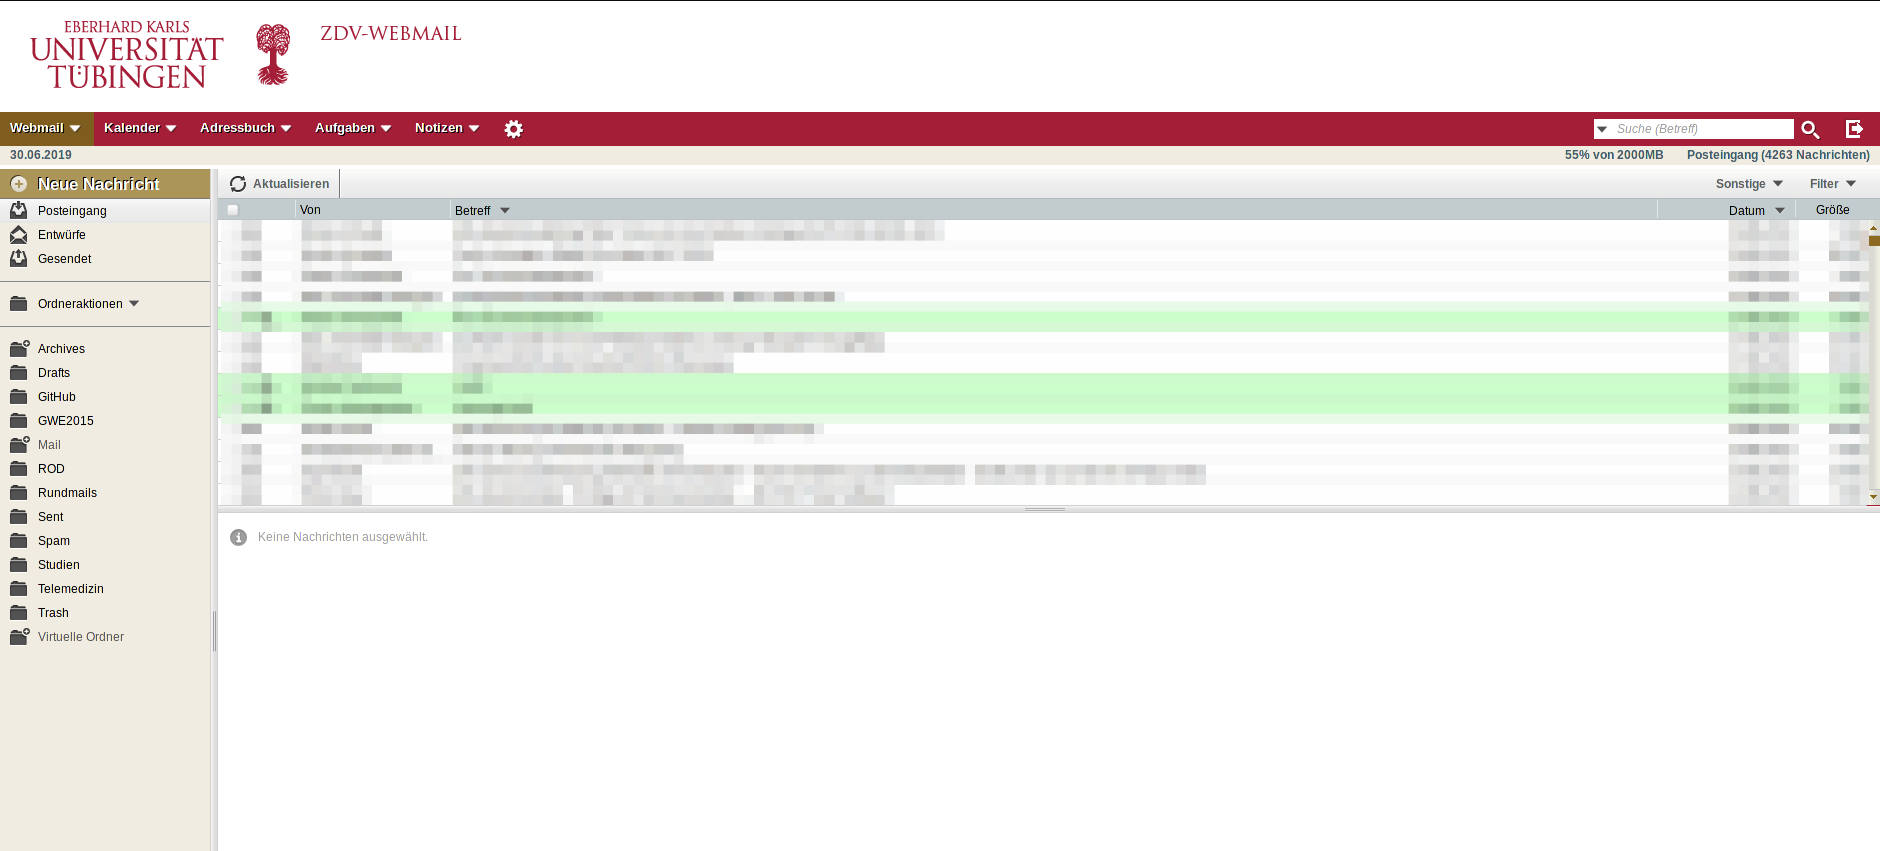
\includegraphics[width=\textwidth]{pictures/webmail.png}
	\end{frame}

	\begin{frame}
	\frametitle{Filterregeln im Webmailer}
	\centering
	\emph{Webmail $\rightarrow$ Filter $\rightarrow \oplus$ neue Regel}\\
	\begin{columns}
		\column[c]{.5\textwidth}
		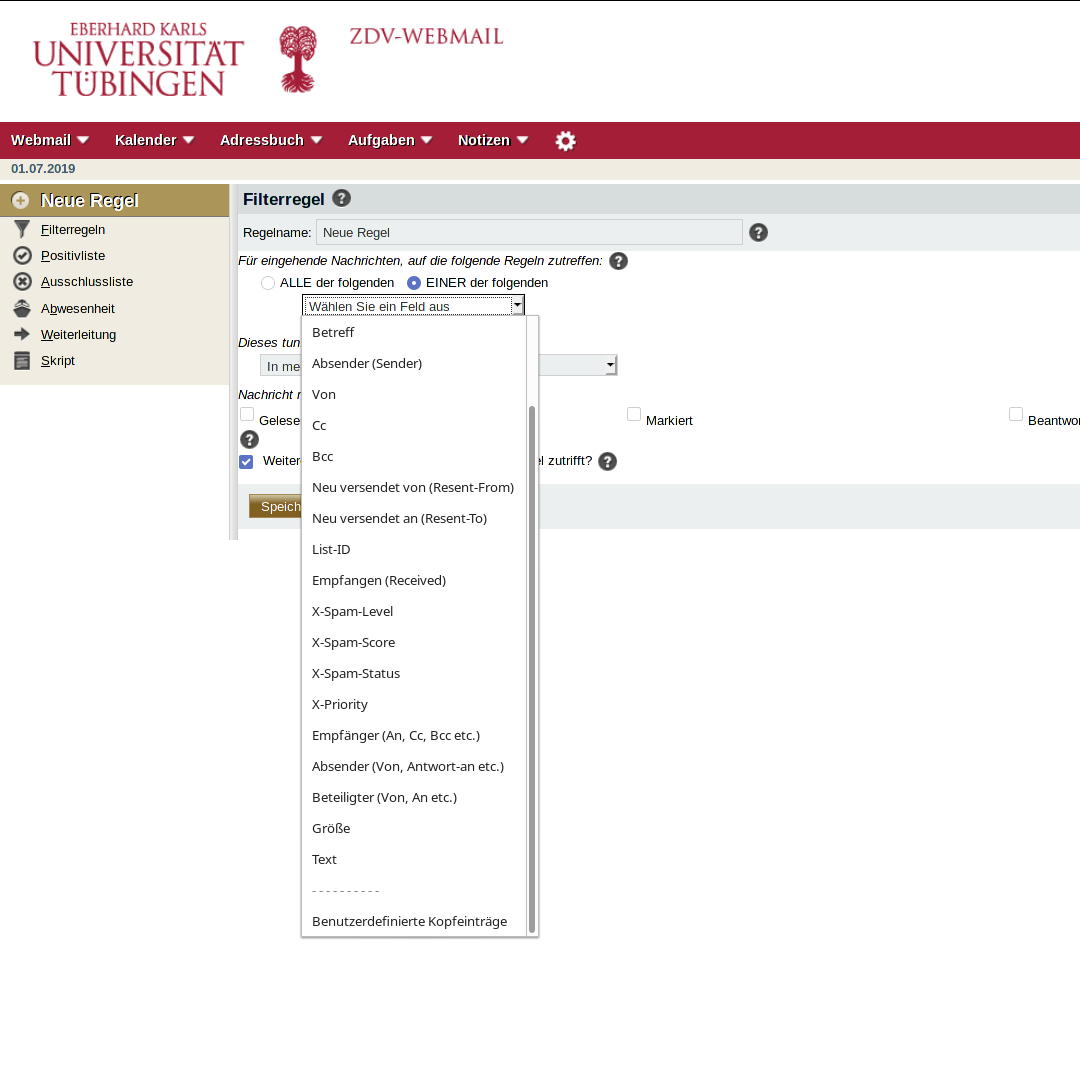
\includegraphics[width=\textwidth]{pictures/filter_dropdown.png}
		\column[c]{.5\textwidth}
		\centering
		Filterung möglich nach:
		\begin{itemize}
			\item Betreff
			\item Empfänger
			\item Inhalt
			\item Sender-Adresse
			\item Wörter im Text
			\item etc.
		\end{itemize}
	\end{columns}
	\end{frame}

	\begin{frame}
	\frametitle{Rundmails filtern: the right way}
	\begin{alertblock}{so nicht}
		\begin{quote}
			
\includegraphics[width=15px]{pictures/quote.png}
			Dies ist eine von der Universitätsleitung genehmigte Rundmail.
		\end{quote}
	Gerade Mails der Uni-Kliniken enthalten diesen Textblock nicht.
	\end{alertblock}
	\begin{exampleblock}{viel besser:}
		Filtern aufrund des Headerfeldes \texttt{X-Comment}
	\end{exampleblock}
	\end{frame}

	\begin{frame}
	\centering
	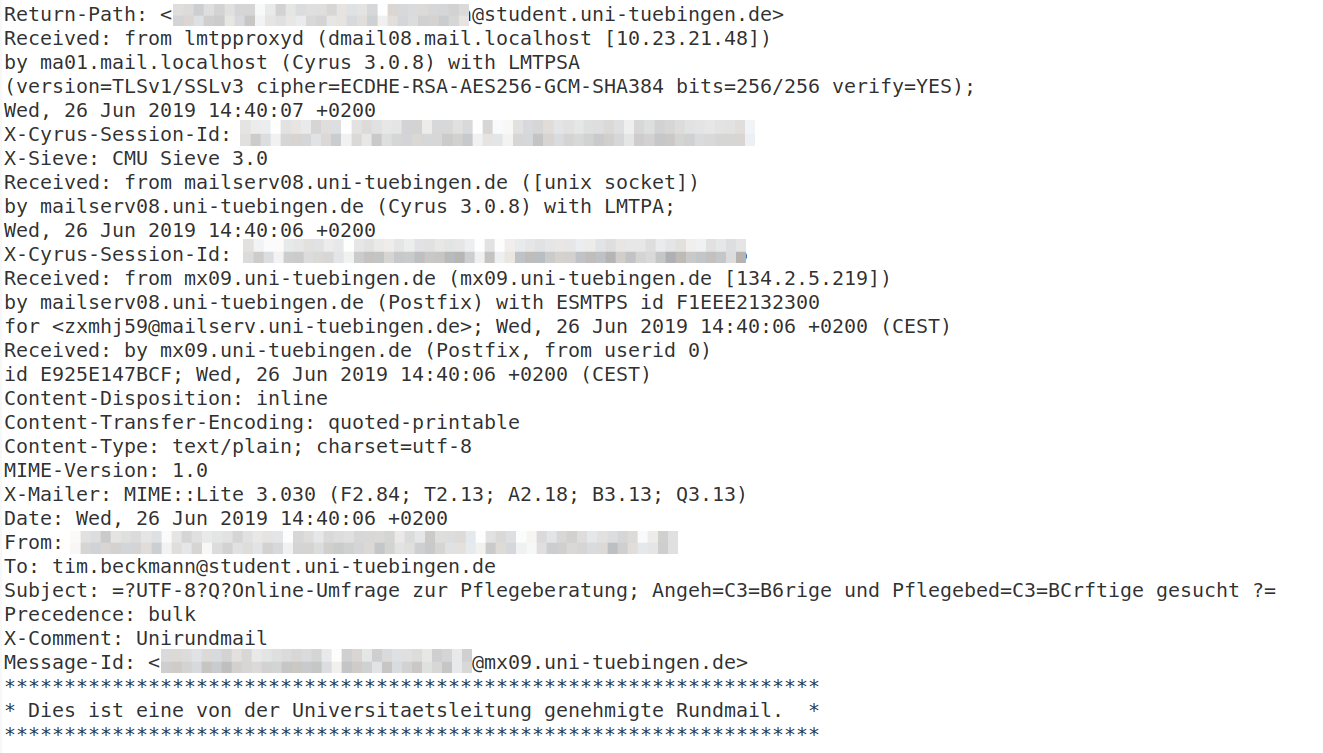
\includegraphics[height=0.8\textheight]{pictures/quelltext.png}
	\end{frame}


\begin{frame}
	\frametitle{Filtern nach Header-Feld X-Comment}
	\centering
	\emph{Im Dropdown-Menü ganz nach unten scrollen, \textbf{Benutzerdefinierte Kopfeinträge} wählen}\\
	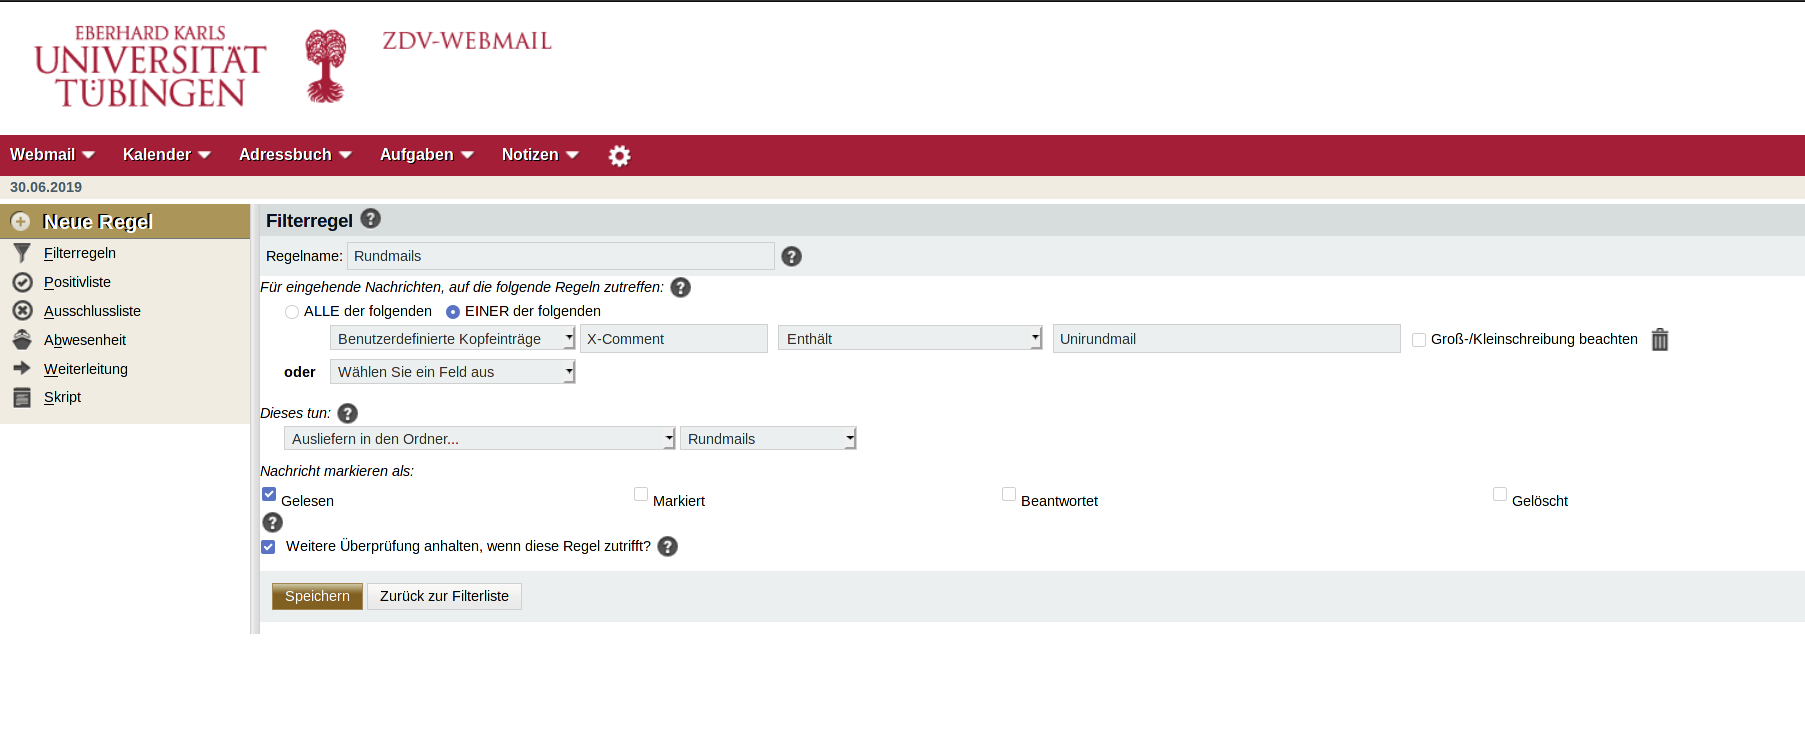
\includegraphics[width=\textwidth]{pictures/filter_regel.png}
\end{frame}

	\begin{frame}
	\frametitle{Weiterleitung an eigene Mail-Adresse}
	\centering
	\emph{Webmail $\rightarrow$ Filter $\rightarrow$ Weiterleitung}\\
	
\includegraphics[width=0.8\textwidth]{pictures/filter_weiterleitung.png}
\end{frame}

	\begin{frame}
	\frametitle{Einrichtung als separates E-Mail-Konto}
	\begin{exampleblock}{Windows/Mac OS/Linux: Thunderbird \quad Android: K-9 Mail}
		Konfigurationsparameter unter \url{https://uni-tuebingen.de/einrichtungen/zentrum-fuer-datenverarbeitung/dienstleistungen/serverdienste/mail/mailserver/}
	\end{exampleblock}
	\end{frame}

	\begin{frame}
	\frametitle{iOS: Autodiscover verwenden}
		\centering
		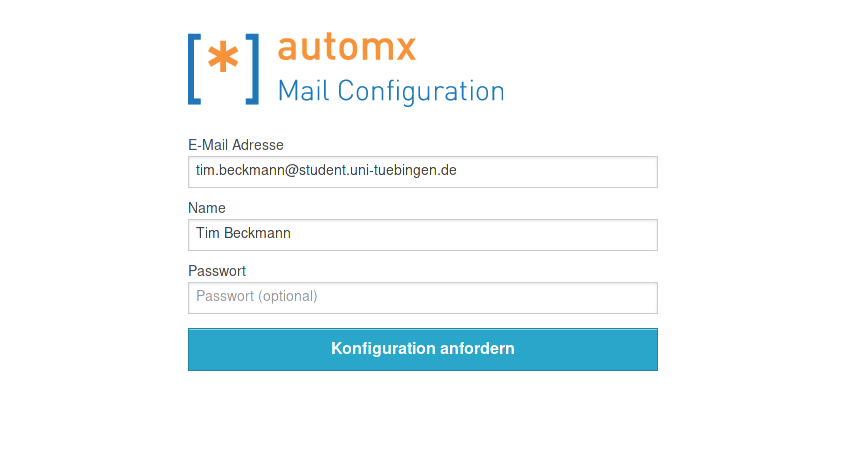
\includegraphics[width=0.5\textwidth]{pictures/autodiscover.png}
		\url{https://autodiscover.uni-tuebingen.de/}
		\begin{alertblock}{ungetestet!}
			(ich besitze keine iOS-Geräte)
		\end{alertblock}
	\end{frame}

	\begin{frame}
		\centering
		\Huge Danke!
	\end{frame}

\end{document}
